\section{Modelling Photometry}
\label{sec:photo}

We use the approach presented in \cite{Vijayan2020} (henceforth \flares\-II) to produce resolved galaxy images, both including and excluding the effects of dust. We first produce spectral energy distributions (SEDs) and then apply top hat rest frame UV and visual band filters to extract photometry. As in \flares\-II we focus on the stellar emission, deferring the treatment of accretion onto the super-massive black holes to a future work. However, as will be shown in the coming sections this simplification does not pose a significant challenge to the results of this work. This approach broadly follows \cite{Wilkins2016a,Wilkins2017,Wilkins2018,Wilkins2020}, with modifications to the dust treatment. For a full description of this method and discussion of the free parameters see \flares\-II. What follows is a brief summary of the approach to compute galaxy images. 

\subsection{Spectral Energy Distribution Modelling}

\begin{figure}
	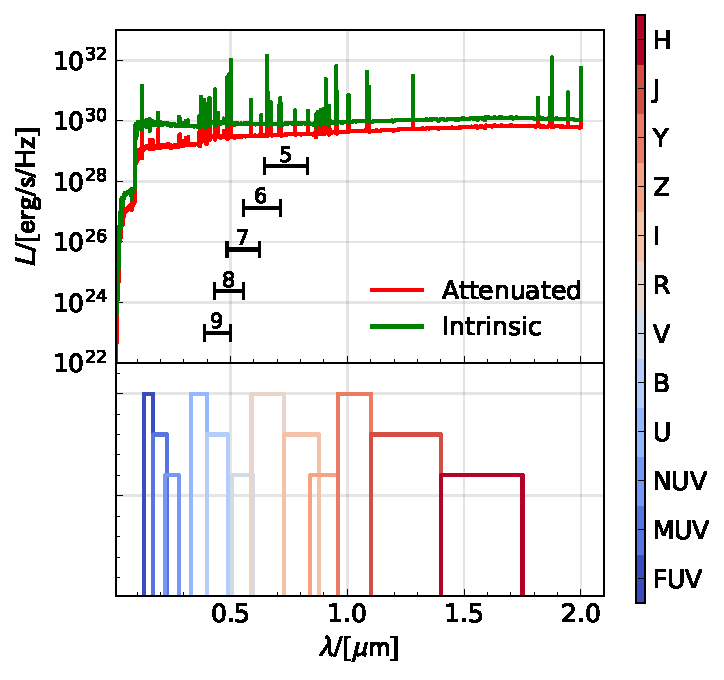
\includegraphics[width=\linewidth]{Figures/SED_sim_default.pdf}
    \caption{The median rest frame SEDs for all galaxies in all \flares\ regions at $z=5$ with $10^{10} \leq M_\star/M_\odot \leq 10^{11.3}$ produced by \texttt{SynthObs}. The top panel shows the intrinsic stellar SED in green and the dust attenuated SED (including Line of Sight effects) in red. The lower panel shows the rest frame top hat photometric filters used throughout this analysis, plotted with an arbitrary $y$ axis to aid interpretation. The black lines correspond to the location and bandwidth of Webb Space Telescope's near-infrared camera's (NIRCam) reddest wide-band filter (F444W) at the indicated redshifts. This indicates the reddest rest frame bands accessible by Webb at high enough resolution to measure robust sizes with NIRCam (0.062 arcseconds) at $z>5$.}
    \label{fig:example_sed}
\end{figure}

In this work we use the \textsc{SynthObs} module\footnote{\href{https://github.com/stephenmwilkins/SynthObs}{github.com/stephenmwilkins/SynthObs}} to produce synthetic rest frame photometry primarily focusing on a top hat far-UV (1500 \AA) filter with a wavelength range of 1300 \AA $\leq \lambda \leq$ 1700 \AA. We do however calculate results for a range of different filters all shown in the example SED in \fig{example_sed}. Each component of the stellar luminosity can be included independently enabling the probing of both the intrinsic luminosity and the effects of dust extinction. In this section we briefly detail each component.

\subsubsection{Stellar Emission}

For the pure stellar emission we start with a simple stellar population model (SSP) by associating each stellar particle with a stellar SED based on the particle's age and metallicity. As with \flares\-II we use v2.2.1 of the Binary Population and Spectral Synthesis (BPASS) stellar population synthesis (SPS) models \citep{BPASS2.2.1} and assume a \cite{chabrier_galactic_2003} Initial Mass Function (IMF). As shown in \cite{Wilkins2016a,Wilkins2017,Wilkins2018} the resulting luminosities are sensitive to the choice of SPS and IMF used in their derivation. 

% \begin{itemize}
%     \item pure stellar emission - v2.2.1 BPASS \cite{BPASS2.2.1}
%     \item Chabrier IMF \cite{chabrier_galactic_2003}
%     \item Cite Steve about IMF effects - \cite{Wilkins2016a,Wilkins2017,Wilkins2018,Wilkins2020}
% \end{itemize}

\subsubsection{Nebular Emission}

To account for the Lyman continuum emission (LyC) of young stellar populations we associate young stellar particles ($t < 10$ Myr, following the assumption from \cite{Charlot_and_Fall2003} that birth clouds dissipate on these timescales) to a $\mathrm{HII}$ region (or birth cloud). To include the LyC emission for each stellar particle we follow the approach detailed in \cite{Wilkins2020}, in which the pure stellar spectrum is processed with the \cloudy\ photoionisation code \citep{Ferland2017} assuming:

\begin{itemize}
    \item The $\mathrm{HII}$ region's metallicity is identical to the stellar particle's.
    \item Dust depletion and relative abundances from \cite{Gutkin2016}.
    \item A reference ionisation parameter (defined at $t=1$ Myr and $Z=0.02$) of $\log_{10}(U_{S,\mathrm{ref}})=-2$.
    \item A hydrogen density of $\log_{10}(n_{\mathrm{H}}/\mathrm{cm}^{-3})=2.5$.
    \item \texttt{CLOUDY}'s default Orion-type graphite and silicate grains.
\end{itemize}

\subsubsection{Dust Attenuation}
\label{sec:dustatt}

To include the effects of dust attenuation from the ISM we adopt a line of sight (LOS) attenuation model. In this model we treat stellar particles as emitters along a line of sight (in this article we select the z-axis of the simulation) and account for the attenuation due to gas particles which intersect this LOS. Using a LOS approach means stellar emission undergoes spatially resolved attenuation rather than the uniform attenuation of a simple screen model, enabling considerably more robust photometry. 

To do this we find all gas particle SPH kernels which intersect the stellar particle's line of sight and integrate along it to get the metal column density, $\Sigma(x,y)$. We then link this metal column density to the ISM dust optical depth in the V-band (550nm), $\tau_{\mathrm{ISM}}(x,y)$, with a similar approach as in \cite{Wilkins2017}. This gives the expression
\begin{equation}
    \tau_{\mathrm{ISM,V}}(x,y) = \mathrm{DTM} \, \kappa_{\mathrm{ISM}} \, \Sigma(x,y),
\end{equation}
where DTM is the galaxy specific dust-to-metal ratio from the fitting function presented in \cite{Vijayan2019}. This is a function of the mass-weighted stellar age ($t$) and the gas-phase metallicity of a galaxy ($Z$),
\begin{equation}
    \mathrm{DTM}=\mathcal{D}_{0} +(\mathcal{D}_{1} - \mathcal{D}_{0})\left[1-\exp\left(-\alpha Z^{\beta}(t/\tau)^{\gamma}\right)\right],
\end{equation}
where $\mathcal{D}_{0}$ and $\mathcal{D}_{1}$ represent the initial type II SNe dust injection and saturation respectively, and $\tau$ is an estimate of the initial dust growth time-scale after dust injection from type II supernovae but prior to the initiation of dust growth on grains
\footnote{For the parameters of this function we use the best fit values from \cite{Vijayan2019} (see Section 4.1.3 therein for further details): $\mathcal{D}_{0}=0.008$, $\mathcal{D}_{1}=0.329$, $\alpha=0.017$, $\beta=-1.337$, $\gamma=2.122$, and $\tau=5\times10^{-5}[\mathrm{Gyr}]/(\mathcal{D}_{0}Z)$.}
The normalisation factor $\kappa_{\mathrm{ISM}}$ was chosen to match the rest frame UVLF from \cite{Bouwens_2015a} and acts as a proxy for dust properties such as average grain size, shape and composition ($\kappa_{\mathrm{ISM}}=0.0795$). The \flares\ simulations do not inherently model dust production and destruction, thus we have to resort to these data driven proxies.  

In addition to attenuation due to the ISM, young stellar populations ($t < 10$ Myr) are still embedded in their birth clouds and thus need to take into account attenuation due to this cloud. For these young stellar particles we include the additional attenuation expression:
\begin{equation}
   \tau_{\mathrm{BC,V}}(x, y)=\kappa_{\mathrm{BC}}(Z/0.01) ,
\end{equation}
where $Z$ is the metallicity of the young stellar particle and $\kappa_{\mathrm{BC}}$ is another normalisation factor encapsulating the dust properties of the birth cloud, for this we assume a constant value of $\kappa_{\mathrm{BC}}=1$. For stellar particles older than $10$ Myr, $\tau_{\mathrm{BC,V}}(x, y)=0$ and there is no contribution.

We then combine these optical depths in the V-band,
\begin{equation}
    \tau_\lambda= (\tau_{\mathrm{BC,V}}+\tau_{\mathrm{ISM,V}}) \left(\frac{\lambda}{550 \mathrm{ nm}}\right)^{-1},
\end{equation}
yielding an expression for the optical depth at other wavelengths which can be applied to the stellar particle SEDs to account for dust attenuation.

% \begin{itemize}
%     \item Additional component from the birth cloud for young stellar particles. Below resolution scale. 
%     \item For particles younger than 10 Myr $\tau_{BC,V}(x, y)=\kappa_{BC}(Z/0.01)$. Again $\kappa_{BC}$ is a normalisation factor but encapsulates the DTM of birthcloud, implying a constant birth cloud DTM. $\kappa_{BC}=1$
%     \item These birth clouds dissipate on this time scale \cite{Charlot_and_Fall2003}.
%     \item We then combine these two contributions to the extinction for a stellar particle.
% \end{itemize}

\subsection{Image creation}
\label{sec:image}

We then apply top hat photometric band filters to the SEDs producing photometry for each stellar particle. Using this photometry we produce synthetic observations with a field of view (FOV) of 60 pkpc x 60 pkpc encompassing the entire 30 pkpc aperture in which a galaxy's integrated quantities are measured (corresponding to 9.34, 12.20, and 14.13 arcseconds at $z=5$, $z=8$ and $z=10$ respectively), see \sec{extract}. We adopt a resolution equal to the redshift dependent softening length of the simulation ($s=2.66 / (1 + z)$ pkpc). 

Synthetic images are often created by treating each stellar particle as a 2-dimensional Gaussian kernel. The standard deviation of this kernel can either be defined by the softening length ($\sigma=s$, producing minimal smoothing), the stellar particle's smoothing length ($\sigma=h_{\mathrm{sml}}$, accounting for the local density), or, most often, the proximity to the $N$th neighbouring stellar particle ($\sigma=r_{\mathrm{N}}$) \cite[e.g.][]{Torrey2015,Ma_18_size,Marshall21}. The full image is then a sum over these contributions. In this method an image ($I$) can therefore be expressed mathematically as
\begin{equation}
I_i =  \exp\left(-\frac{(X-x_i)^2 + (Y-y_i)^2}{2\sigma_{i}^2}\right),
\end{equation}
\begin{equation}
I = \sum_{i=0}^{N_\star} \frac{I_i L_i}{\sum_{\mathrm{pix}}I_i},
\end{equation}
where $I_i$ is the smoothed image (kernel) produced for the $i$th stellar particle, $\sigma_i$ is the standard deviation of the $i$th stellar particle's kernel, $X$ and $Y$ are a grid of pixel positions, $x_i$ and $y_i$ are the $i$th stellar particle's x axis and y axis positions in the desired projection, $L_i$ is the luminosity of the $i$th particle, and the sum in the denominator is a sum over all pixels for the $i$th stellar particle to normalise the kernel. 

However, this approach not only differs from the SPH treatment of a stellar particle but is also extremely computationally expensive. Unless artificially truncated a Gaussian kernel encompasses the whole image, leading to insignificant but time consuming calculations. 
In fact, in SPH simulations a stellar particle is treated as a representation of a fluid with the full extent of the stellar population described by a spline kernel with a definitive cut off where the kernel falls to 0 \citep{Borrow2021}. Using a spline kernel based approach is not only a better representation of the underlying simulation's treatment of stellar particles but also greatly reduces the size of the computation by limiting the number of pixels computed per stellar particle.

For these reasons we implement a method of smoothing employing the SPH kernel used in the simulation to describe a stellar particle's `extent'. In the \textsc{Anarchy} SPH scheme, used in the EAGLE model \citep{schaye_eagle_2015}, this kernel is the $C_{2}$ Wendland kernel \citep{wendland_piecewise_1995, Dehnen2012}. We therefore adopt this kernel in this work, but note that for other simulations the kernel corresponding to that particular simulation should be used to maximise the fidelity of this method.

As with the Gaussian approach, an image can be described as a sum over kernels; unlike the Gaussian approach however, the spline kernels are necessarily 3-dimensional and need projecting into the $x-y$ plane. To achieve this we calculate the spline kernels on a voxel grid and sum over the $z$-axis,  
\begin{equation}
I =  \sum_{z\mathrm{-axis}}\sum_{i=0}^{N_{\star}} \frac{K_i}{\sum_{\mathrm{vox}} K_i}L_i,
\end{equation}
where each stellar particle's kernel ($K_i$) is now
\begin{equation}
K_i =  \frac{21}{2\pi} \frac{w_i}{h_{\mathrm{sml}}^3},
\end{equation}
with the kernel $w_i$ given by
\begin{equation}
        w_i(q_i=r/h_i) = 
\begin{cases}
    \left(1-q_i\right)^{4}\left(1+4q_i\right), & q_i \leq 1\\
    0,              & q_i > 1
\end{cases},
\end{equation}
where $r$ is the distance between the particle and any given voxel within the kernel. 

To compute this kernel efficiently we employ a KD-Tree algorithm, building a tree based on voxel coordinates. We query the tree for all non-zero pixels where the distance between the pixel and the stellar particle ($r$) is less than the limits of the smoothing kernel (here $r<h$), greatly reducing the computation from $O(N_\star N_{\mathrm{pix}})$ in the Gaussian case to $O(N_\star N_{\mathrm{vox}(r<h)})$ using the more representative spline approach.


\begin{figure*}
	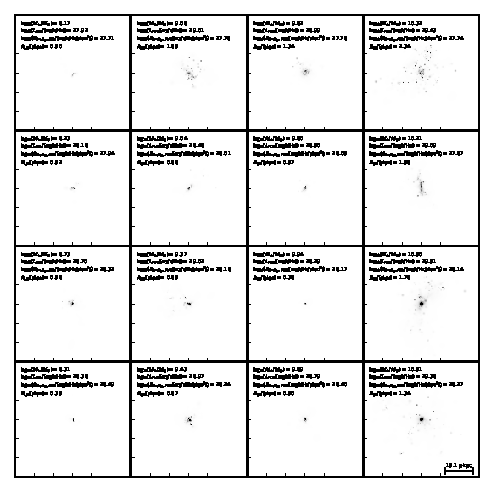
\includegraphics[width=\linewidth]{Figures/ImgGrid_FAKE.TH.FUV_5.0_14_010_z005p000_sim_Total_default.pdf}
    \caption{A subset of $z=5$ synthetic far UV galaxy images computed using the method outlined in \sec{image}. Each panel is the full 60 pkpc x 60 pkpc FOV for each galaxy. Galaxies increase in mass left to right and increase in central surface density top to bottom. The pixel values of these images are linearly normalised across all panels with their mass, luminosity, central surface density and half light radius included in each panel. The galaxies included in this subset were randomly selected from each mass and central surface density bin, even so they display the variety of morphologies already present by $z=5$ in \flares.}
    \label{fig:example_img}
\end{figure*}

In \fig{example_img} we present a grid of randomly selected galaxy images in the far-UV filter along with their stellar mass (derived by summing the underlying particle distribution), luminosities, central surface densities and half light radii measured including the effects of dust. It should be noted that throughout this analysis we do not rotate galaxies, instead adopting their existing orientation in the box to emulate the stochastic viewing angles of galaxies in the real Universe. Henceforth, all analysis derived from images will use this method of stellar particle smoothing (implemented from \sec{pixel} onwards), unless explicitly stated otherwise. In \app{smooth} we present comparisons between the Gaussian and spline approach for this simulation. 